\documentclass[11pt,twocolumn,letterpaper]{article}

% \usepackage[review]{cvpr}      % To produce the REVIEW version
\usepackage{cvpr}              % To produce the CAMERA-READY version
% \usepackage[pagenumbers]{cvpr} % To force page numbers, e.g. for an arXiv version

\usepackage{graphicx}
\usepackage{amsmath}
\usepackage{amssymb}
\usepackage{booktabs}
\usepackage[pagebackref,breaklinks,colorlinks]{hyperref}
\usepackage[capitalize]{cleveref}
\crefname{section}{Sec.}{Secs.}
\Crefname{section}{Section}{Sections}
\Crefname{table}{Table}{Tables}
\crefname{table}{Tab.}{Tabs.}
\setcounter{figure}{3}

\def\cvprPaperID{1} % *** Enter the CVPR Paper ID here
\def\confName{1}
\def\confYear{1}

\begin{document}
\title{Appendix}

\maketitle
\thispagestyle{empty}

\section{Knowledge Graph}
Making predictions for the spread of the COVID-19 pandemic is a complex task, which can benefit from the information available from multiple sources. To integrate this information into the multi-variate time series models, we can build a knowledge graph using all the information and use the knowledge graph to create embeddings that can be used with the time series models. Using knowledge graphs can improve the situational awareness of the models as we incorporate more information from the real-world and thus producing more accurate and robust forecasts.

\subsection{Building knowledge graph}
Building the knowledge graph consists of defining a schema and updating the knowledge graph dynamically. For building the schema we need to first identify how the knowledge graph embeddings are going to integrate with the time-series models. For example, are we going to use the embeddings of "date" or "state" or even multiple variables when integrating with the time-series models? These variables will act as a bridge between the information stored in the knowledge graph and the information used by the time-series models.

After identifying these bridge variables, we can start working on creating a schema for the knowledge graph. The goal of this step is to structure the schema around these variables so that these variables can transfer as much information as possible from the knowledge graph to the time-series models. For variables, like "date" this is easy as most of the data should already be dated. For variables that cannot be directly connected to the bridge variables, we have to look into the number of hops necessary to reach these bridge variables. The greater the number of hops, the lesser the chances of information being transferred from the embeddings to the time-series models and vice versa. After integrating the knowledge graph with the time-series models, future research can look into the impact of the number of hops on the performance of the time-series models.

The knowledge graph also needs to be temporal i.e. changing with time, meaning as new data comes in the knowledge graph is updated resulting in new embeddings. The reason for doing this is to prevent any data leakage from using future sources of data in the knowledge graph, which can overfit the time-series model. In practice, this is done by first creating the knowledge graph till a specific date. Then in the next step, we add data for the next date and repeat. When using temporal graphs we can add an auxiliary unsupervised task of predicting the graph structure in the next step, along with any existing supervised task, as multi-task learning has been shown to benefit computer vision and natural language processing tasks, and we can incorporate these into the graph domain also.

\subsection{Creating Embeddings}
In the previous section, we defined a schema and created a temporal knowledge graph. This step can be done in Neo4j (or Scalation in the future) which provides a tested knowledge graph database. Using Neo4j, we can define the schema and load the necessary data and then use one of the built-in methods (like GraphSage) to train embeddings which can be passed to the time-series models.

Specifically, every node is associated with an N-dimensional vector and every edge is associated with an R-dimensional vector, which will be learned by a model. Models like GraphSage, ComplEx, and TransE will take these vectors as inputs and modify them to minimize the specified loss function. Internally, these models build upon the message-passing algorithm where a node first collects information from all the neighboring nodes and then passes it further. The model aims to learn embeddings that best capture the graph structure, meaning captures the maximum amount of information from the knowledge graph to the embedding vectors.

\begin{figure*}
\centering
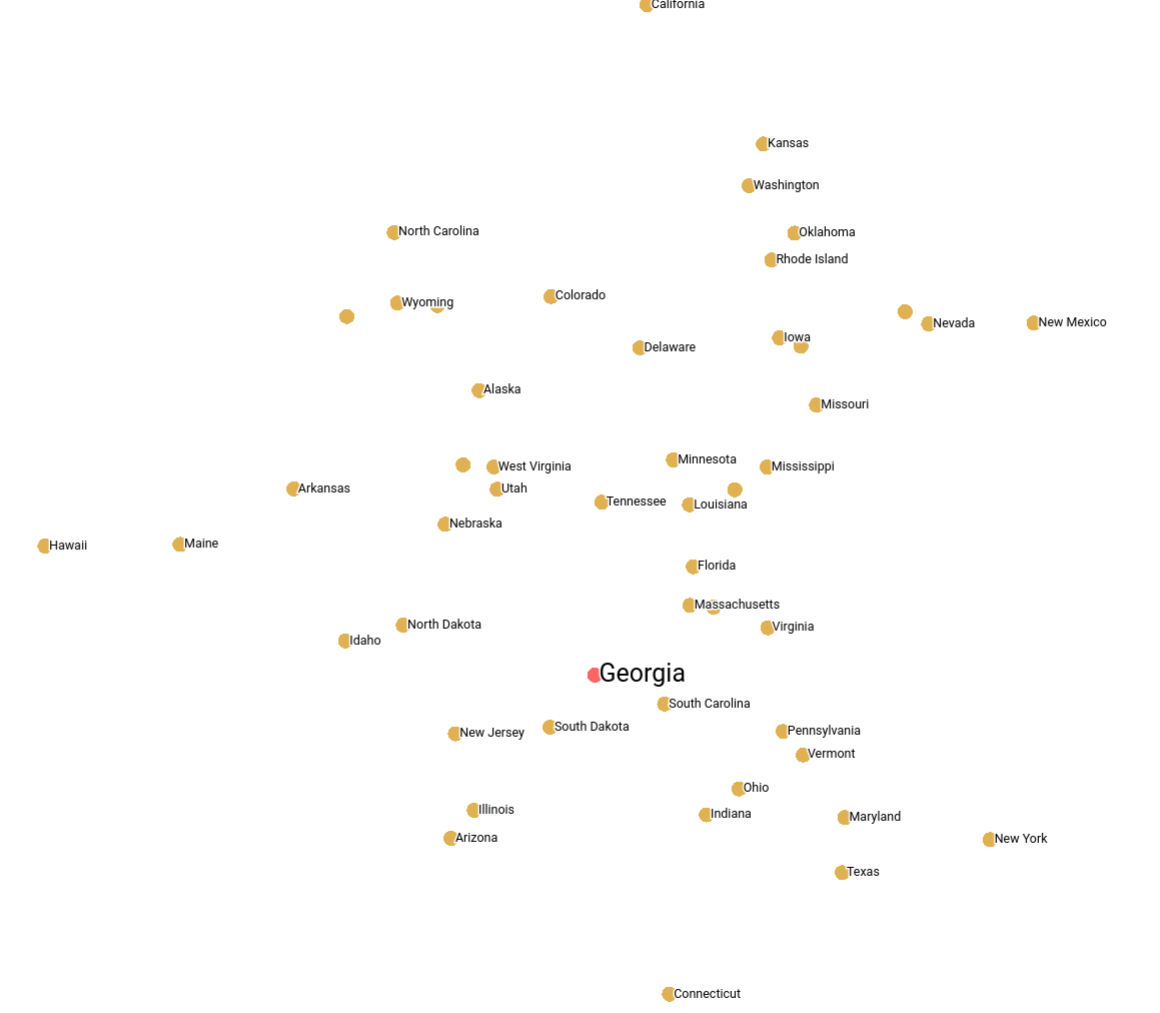
\includegraphics[width=\linewidth]{images/embeddings.png}
\caption{2D projection of the state embeddings obtained from the knowledge graph using PCA. States that are closer to each other share similar COVID-19 patterns as learned by the models from the knowledge graph. To verify the quality of the  embeddings we cannot simply look at the figure, because it is not possible to differentiate these embeddings from random embeddings. And thus we have to pass the embeddings to the time series model and see if the metrics improve.}
\label{figure4}
\end{figure*}

An example of the learned embeddings is shown in \cref{figure4} where we visualize the 2D embeddings\footnote{\href{https://projector.tensorflow.org/}{https://projector.tensorflow.org/} is used to get the visualization}. Using the figure, we can look at individual states and the states that are closer to each other share similar COVID-19 patterns as learned from the knowledge graph. The embeddings projection cannot be used to verify the quality of the knowledge graph, as it is not possible to differentiate from random embeddings. So the only way to evaluate the quality of the embeddings obtained from the knowledge graph is to pass them to the time series model and see if the metrics improve.

\subsection{Integrating with time-series models}
Bridge variables are used to integrate the knowledge graph and the input for the time-series models. Since bridge variables are generally categorical like date, and state which are usually initialized as random/one-hot-encoded embedding vectors, we can directly replace these with the embeddings learned from the knowledge graph and pass them as input to the time-series models. To reduce the noise in the embeddings, the embeddings can be projected to a lower latent space using UMAP, T-SNE, or PCA.

\end{document}
